\chapter{Ingeniería del Software y Herramientas}

\section{Metodología de Ingeniería del Software}

Para el desarrollo de este software, era clave establecer un orden ante las múltiples tareas a realizar. En base a esto, el modelo de desarrollo incremental fue la mejor metodología a seguir. La idea era subdividir las tareas en procesos, teniendo cada una sus correspondientes fases de análisis, diseño, código y prueba, como se puede apreciar en la figura \ref{fig:modeloincremental}.

\begin{figure}
	\centering
	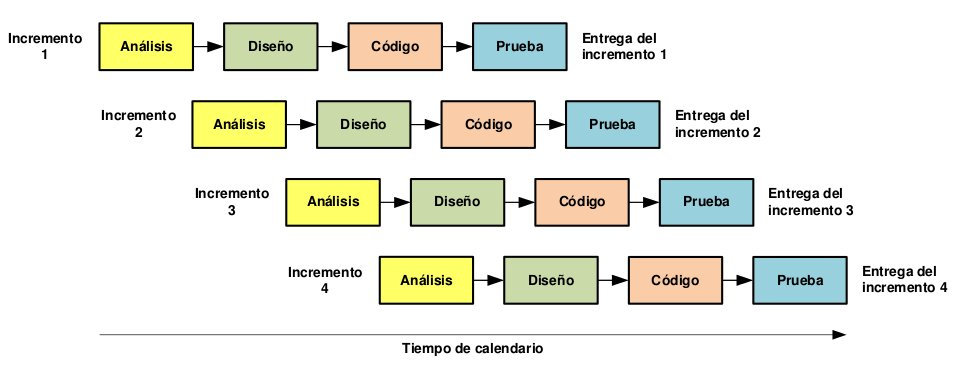
\includegraphics[width=1\linewidth]{imagenes/modelo_incremental}
	\caption{Imagen de la estructura del modelo incremental \cite{modeloIncremental}}
	\label{fig:modeloincremental}
\end{figure}

Este tipo de metodología permite realizar desarrollos o tareas en paralelo, para al final unirlo todo y que funcione correctamente. Una estructura así era necesaria, ya que para implementar cada uno de los gráficos disponibles, necesitaba su propio análisis, su adaptación del diseño original al de la aplicación, aplicar las técnicas de reducción apropiadas para cada gráfico, y su correspondiente tiempo de pruebas.

\section{Planificación}

Como se ha explicado en el apartado anterior, al seguir una metodología incremental durante el desarrollo de la API, permite agrupar las tareas en desarrollos independientes.

La primera tarea fue realizar el diseño base del circuito funcional de la herramienta, es decir, cual era la función de cada una de las herramientas que se iban a implementar y como se conectaban con el resto, para así lograr obtener un flujo de interacción entre todas. Establecido el diseño, el siguiente paso sería implementarlo y comprobar que el flujo de datos entre todas las aplicaciones y el resultado obtenido era el correcto.

Otra de las tareas que se desarrollaron el paralelo con el resto era el diseño de la lista de gráficos disponibles. Con el uso de la librería de gráficos D3JS, que se explicará más adelante, el siguiente paso era elegir que gráficos se iban a implementar, adaptarlos a la API y comprobar que se dibujaran correctamente.

También otra tarea importante fue el desarrollo de la interfaz web de la API. Diseñar una buena interfaz capaz de aprovechar la máxima potencia del núcleo de la aplicación, era una de las prioridades básicas. Con ella se puede acceder a todas las funciones de la API, configurar las distintas conexiones con las herramientas principales como \textit{MongoDB} \cite{MongoInicial}, \textit{Spark} o \textit{Hadoop} de manera sencilla, o tener la posibilidad de visualizar varios gráficos resultados para poder comparar entre ellos y mejorar el análisis de los datos.

La parte de testeo de la aplicación para comprobar los límites de la misma, fueron casi tres semanas de pruebas. En ella hubo que probar el rendimiento de la aplicación en situaciones reales, con grandes cantidades de datos, y comprobando el tiempo que podía tardar en procesarlo, si no había ningún error.

\section{Lenguajes de Programación y Herramientas}

Durante cada una de las tareas en cada fase, ha habido que aprender a utilizar herramientas y aprender programar en lenguajes, como es el caso de HTML, CSS y Javascript, para poder crear una interfaz web que se adapte a las funciones de la API, o como el caso de \textit{Scala}, lenguaje para programar las funciones de \textit{Spark}.

\subsection{Scala}
\begin{minipage}{\textwidth}
	\centering
	
\includegraphics[width=0.3\textwidth]{imagenes/scala_logo.jpg}\\[0.1cm]
\end{minipage}

Uno de los lenguajes más novedosos es \textbf{Scala}. Es un lenguaje de programación multi-paradigma cuya base está diseñada para programar con patrones. Además integra características de los lenguajes orientados a objetos y funcionales como Java \cite{ScalaInicial}. Al ser un lenguaje funcional, Scala permite desarrollar en una sintaxis ligera, definiendo funciones para realizar las operaciones e incluso anidarlas. 

Scala está basado en el paradigma MapReduce, que se comentó al comiendo del documento. Esto quiere decir que todos los procesamientos los puede realizar de manera paralela, aumentando la velocidad de cómputo.

Por todas las grandes características que ofrece, es el lenguaje elegido para programar las funciones de Spark, de entre todos los disponibles de la herramienta. Está perfectamente integrado con Spark y permite que la programación que se realice, sea muy escalable, tanto si se ejecuta sobre un ordenador como sobre un cluster, sin necesidad de cambiar nada de lo programado. 

En la API, se han programado en Scala todas las funciones de análisis de los datos que provienen de Hadoop, aplicando las técnicas de reducción de datos y esquemas de agrupación elegidos para el gráfico que se está desarrollando. Se adapta muy bien a la lectura de datos de tipo CSV o JSON, tipos de datos principales en la base de datos. 


\subsection{NodeJS}
\begin{minipage}{\textwidth}
	\centering
	
\includegraphics[width=0.4\textwidth]{imagenes/nodejs_logo.png}\\[0.1cm]
\end{minipage}

En la parte intermedia del diseño se encuentra \textbf{NodeJS} \cite{NodeJSInicial}. Está desarrollado en el lenguaje Javascript. Es un entorno de ejecución que gestiona las llamadas que se producen de manera asíncrona \cite{NodeJSAbout}. Esto permite manejar varias conexiones de manera concurrente sin la necesidad de que el usuario esté vigilando el bloqueo de procesos, como ocurre en las operaciones de redes basadas en hilos o hebras. Debido a que no hay bloqueos, es muy sencillo crear aplicaciones escalables en NodeJS.

Node mejora el modelo de eventos diseñados en otros sistemas, tratando el bucle de eventos como un entorno en vez de una librería. Su comportamiento se define a través de funciones callbacks, las cuales al inicio y final del script se inicia el servidor. En otros lenguajes, en las funciones callback se realiza una llamada de bloqueo, pero en NodeJS la añade al bucle de eventos después de ejecutar el script de entrada. Sale del bucle cuando no hay más funciones callbacks que ejecutar. Se puede apreciar un gráfico explicativo en la figura \ref{fig:nodejseventloop}.

\begin{figure}
	\centering
	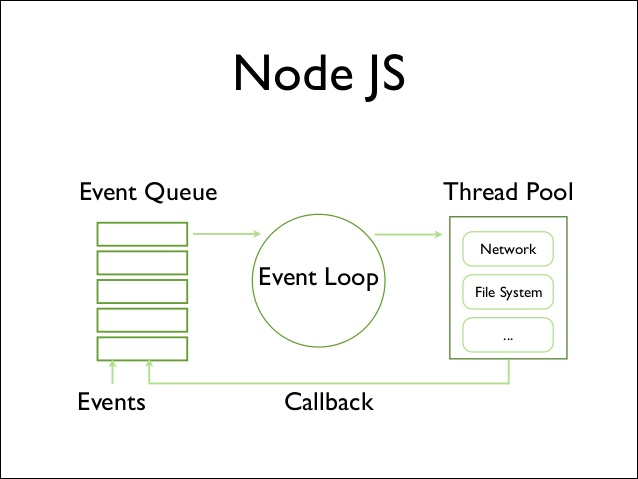
\includegraphics[width=0.9\linewidth]{imagenes/NodeJS_Event_Loop}
	\caption{Esquema del bucle de eventos de NodeJS \cite{NodeJSEventLoop}}
	\label{fig:nodejseventloop}
\end{figure}

Para la API desarrollada, NodeJS es una parte importante del sistema. Es la capa intermedia de la aplicación, donde se encarga de la comunicación entre la interfaz web del usuario con Hadoop, Spark y MongoDB. 
Además, se encarga también de configurar el servidor virtual donde se gestionan todas las peticiones. En este servidor se recogen las peticiones de representar un gráfico concreto, para unos datos y con unos parámetros específicos. Después se encarga de mandar a Spark la información solicitada por el usuario y, a continuación, espera a que el resultado esté disponible en MongoDB. Este se almacena en una base de datos en formato JSON, como ya se explicó en el apartado correspondiente a Mongo. Una vez obtenido, se encarga de dibujar el gráfico usando la librería D3JS.

\subsection{D3JS}
\begin{minipage}{\textwidth}
	\centering
	
\includegraphics[width=0.5\textwidth]{imagenes/d3js_logo.png}\\[0.1cm]
\end{minipage}

\textbf{D3JS} \cite{D3JSGithub} es una librería escrita en Javascript encargada de producir gráficos interactivos a partir de documentos basados en datos, como los ficheros de tipo CSV, TSV o JSON. La base para representar los gráficos de la librería D3JS es utilizar SVG, Canvas y HTML. Al estar escrito en Javascript, el lenguaje para darle funcionalidad a las páginas web, D3JS tiene la potencia para poder interactuar con los gráficos diseñados. De esta manera, las funciones de la librería permiten crear objetos de tipo SVG, darle efectos dinámicos o agregar información sobre el gráfico, o incluso seleccionar algunos de los elementos del infograma, pudiendo obtener otro como resultado de esa selección. 

D3JS se ha implementado como la librería para crear los gráficos de la API. En este caso, cada uno de los gráficos se genera a partir de obtener los resultados de los cálculos por parte de Spark, que están almacenados en MongoDB. Si bien, cada uno de los gráficos tiene puntos fuertes y débiles, por lo que es imprescindible la mano de un usuario experto en análisis de datos, para saber qué gráfico es el adecuado para los datos seleccionados a representar y con qué parámetros. Así se podrá obtener buenos resultados, que sean capaces de expresar lo que están contando los datos, ya que también es parte fundamental saber interpretar los infogramas.

\subsection{HTML, CSS y Javascript}
\begin{minipage}{\textwidth}
	\centering
	
\includegraphics[width=0.3\textwidth]{imagenes/HTML5_CSS_JavaScript_logo.png}\\[0.1cm]
\end{minipage}

Al estar escrita en Javascript la librería D3JS, lo mejor para aprovechar toda su potencia es crear una interfaz web para los usuarios finales. Esto permite poder acceder al sistema desde cualquier parte del mundo, desde cualquier dispositivo, de manera rápida y sencilla, a la vez que escalable. 

Con esta idea en mente, lo primordial es crear una interfaz que aproveche el máximo rendimiento de la aplicación, con un diseño elegante y sencillo. Para ello, se utilizó la plantilla \textbf{Gentelella} \cite{GentelellaGithub}, la cual incorpora muchas posibilidades para diseñar la web y una amplia gama de funcionalidad para cada uno de los paneles. 
Es una de las plantillas gratuitas que mejor se adapta a dispositivos tanto móviles como tablets. Además, trae varia funcionalidad para gestionar usuarios, lo que permite implementarlo en un futuro como una gran mejora del programa.


\subsection{GitHub}
\begin{minipage}{\textwidth}
	\centering
	
\includegraphics[width=0.4\textwidth]{imagenes/github_logo.png}\\[0.1cm]
\end{minipage}

Una de las herramientas fundamentales para todos los proyectos, es el gestor de versiones \textbf{GitHub}. Con ello se puede controlar cada una de las actualizaciones que se realizan del sistema, dando la posibilidad de volver atrás para comprobar cualquier estado anterior del mismo. Además permite gestionar las tareas a desarrollar mediante los \textit{Milestones}, reportar errores de funcionalidad, añadir mejoras a la aplicación o documentar cada una de las tareas. Pero la gran ventaja es que permite que otra gente pueda colaborar en el proyecto o controlar el proceso de desarrollo. 

Todas estas características han sido utilizadas durante el desarrollo de la API, haciendo más sencilla el control sobre la misma. También cabe destacar, que GitHub ha servido de puente para las actualizaciones entre los desarrollos en el ordenador local y el servidor donde se aloja el sistema.

\subsection{Docker}
\begin{minipage}{\textwidth}
	\centering
	
\includegraphics[width=0.4\textwidth]{imagenes/docker_logo.png}\\[0.1cm]
\end{minipage}

\textbf{Docker} \cite{DockerInicial} es una plataforma abierta, usada por desarrolladores y administradores de sistemas, para desplegar aplicaciones dentro de contenedores aislados del sistema operativo.
Para realizar el desarrollo y pruebas correspondientes de la API, se ha utilizado Docker como herramienta para desplegar el sistema en los servidores de la ETSIIT durante todo el proceso.

\subsection{Lucidchart}
\begin{minipage}{\textwidth}
	\centering
	
\includegraphics[width=0.4\textwidth]{imagenes/lucidchart_logo.png}\\[0.1cm]
\end{minipage}

\textbf{Lucidchart} \cite{LucidchartInicial} es una herramienta para el diseño de diagramas de flujo a nivel profesional. Permite compartir los diseños para colaborar entre usuarios en tiempo real. Se pueden crear desde diagramas de flujo hasta diseños UML, pasando por una amplia variedad de tipos de diagramas. 

En esta ocasión, se ha utilizado Lucidchart para el diseño de la mayoría de las figuras de este documento donde se explica algunos de los funcionamientos del sistema. 

\subsection{LaTeX}
\begin{minipage}{\textwidth}
	\centering
	
\includegraphics[width=0.3\textwidth]{imagenes/latex_logo.png}\\[0.1cm]
\end{minipage}

\textbf{LaTeX} es un sistema de composición de textos orientado a la gran calidad tipográfica. Debido a esta característica y sus amplias posibilidades (por ejemplo, facilidad de escritura de expresiones matemáticas) es muy usado en el ámbito científico y académico. Por esta razón,  TeXstudio \cite{TexstudioInicial} ha sido el editor de texto seleccionado para escribir este documento LaTeX.



